%"Nødvendige pakker" (copilot fiksa):
\documentclass[a4paper,11pt, norsk]{article}
\usepackage[utf8]{inputenc}
\usepackage[norsk]{babel}
\usepackage{amsmath}
\usepackage{amsfonts}
\usepackage{amssymb}
\usepackage{graphicx}
\usepackage{float}
\usepackage{hyperref}
\usepackage{listings}
\usepackage{color}
\usepackage{subcaption}
\usepackage{tikz}
\usepackage{pgfplots}
\usepackage{pgfplotstable}
\usepackage{booktabs}
\usepackage{multirow}
\usepackage{multicol}
\usepackage{enumitem}
\usepackage{mathtools}
\usepackage{algorithm}
\usepackage{algpseudocode}
\usepackage{url}
\usepackage{pdfpages}
\usepackage{caption}
\usepackage{subcaption}
\usepackage{listings}
\usepackage{color}
\usepackage{tikz}
\usepackage{pgfplots}
\usepackage{pgfplotstable}

%Begynnelsen av dokumentet
\begin{document}
\title{TDT4145, Prosjekt del 1}
\author{Gruppe 158: Erik Dudek, Einar Rye, Ida Høyland}
\maketitle

%Innholdsfortegnelse som heter innholdsfortegnelse:
\tableofcontents

\newpage{}

\section{ER-modell}
\begin{figure}[H]
\centering
\noindent\makebox[\textwidth]{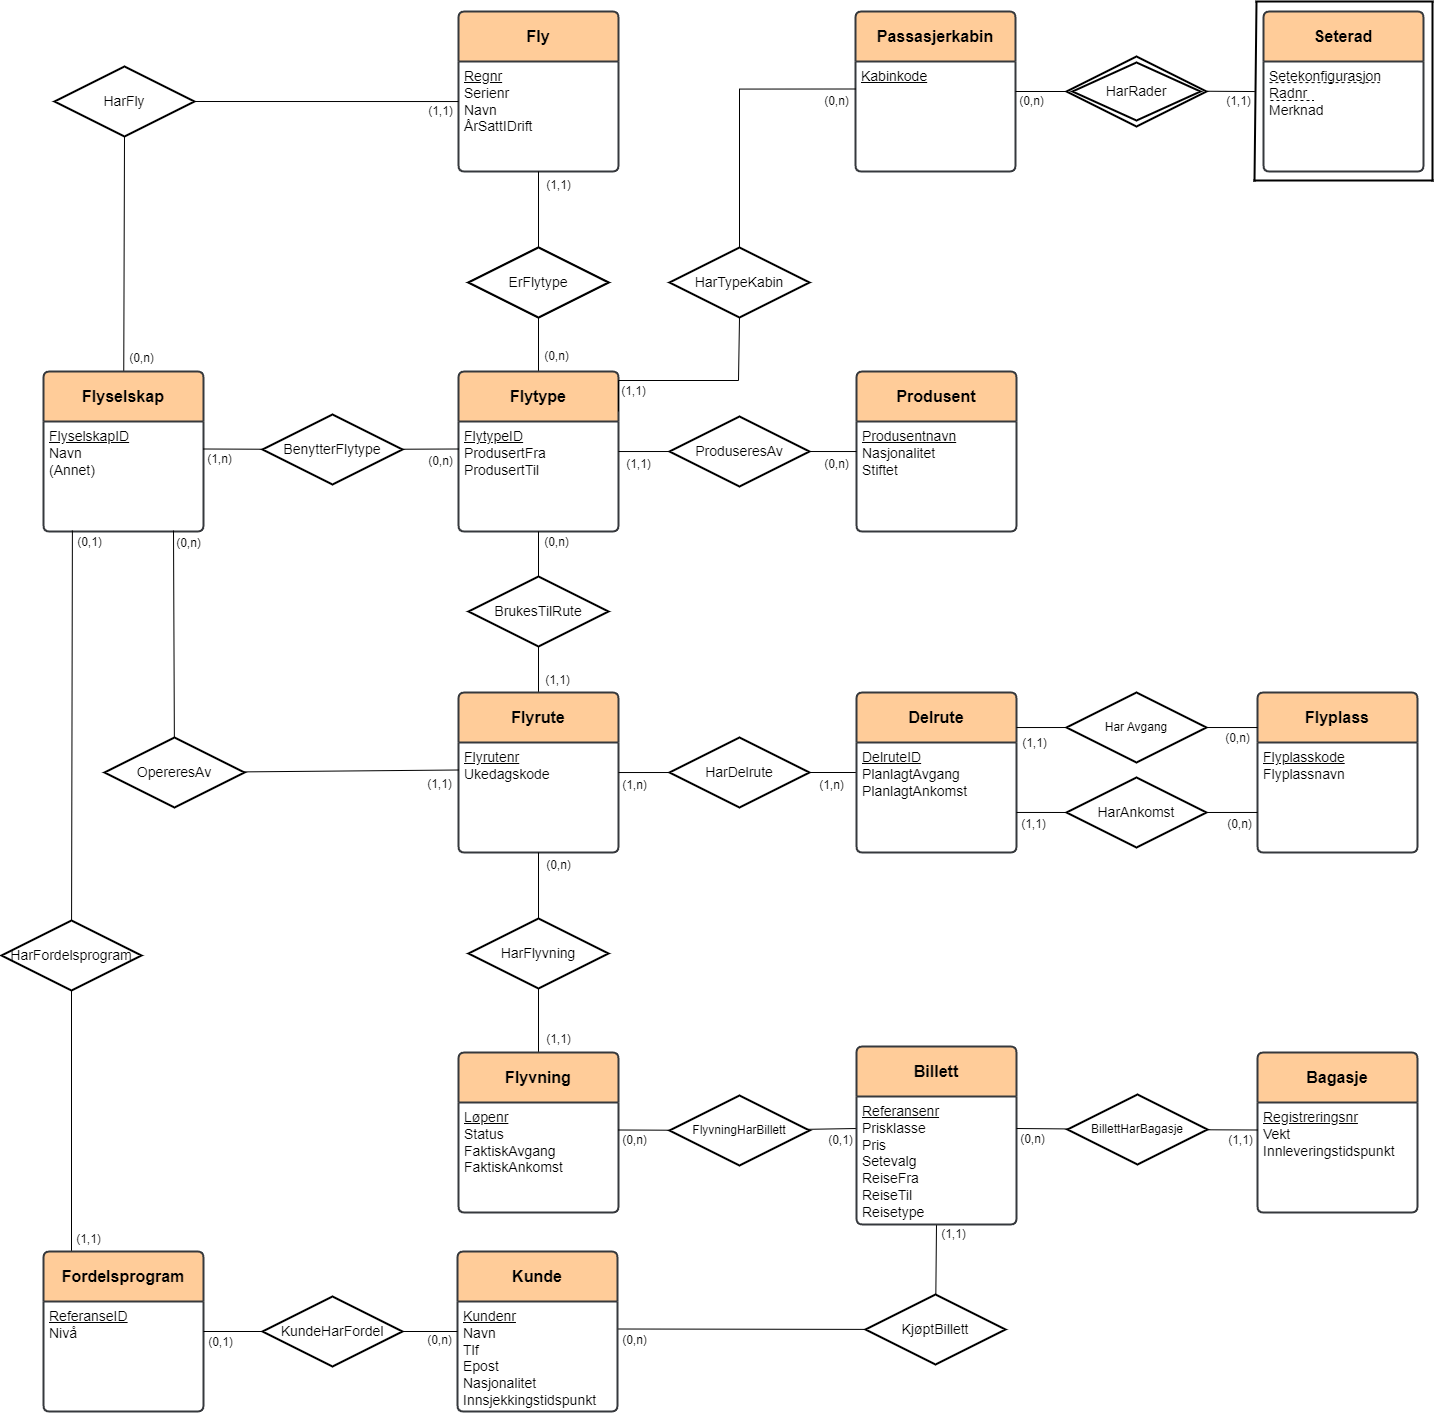
\includegraphics[width=0.9\paperwidth]{figurer/ER-modell.png}}
\end{figure}
\newpage{}

\subsection{Forutsetninger}
\begin{itemize}[noitemsep,topsep=0pt,parsep=0pt,partopsep=0pt]
\item Entiteten Fly har en unikt identifiserende nøkkelatributt Regnr og et Serienr som kun er unik for produsenten av et fly. Derfor er \mbox{Serienr} satt som en normal attributt og det forutsettes at unikheten til \mbox{dette} attributtet opprettholdes i implementasjonen av databasen ved en \mbox{begrensning}.  
\item Entiteten Flyplass har Flyplasskoden som primærnøkkel og Flyplassnavn som normalattributt. Sistnevnte skal være unik og må implementeres med en begrensning.
\item For å gjøre en billettbestilling til en flyvning må status være 'planned' som vi forutsetter kan legges inn som en begrensning i oppretningen av databasen eller opprettholdes manuelt av databasens bruker. 
\item Dersom en flyrute består av to eller flere delruter, kan man kjøpe delrutene for seg. Hver delrute vil da ha en pris. Prisen på hele flyruten vil være
mindre enn summen av prisen på alle delrutene. 
\item En billett kan gjelde for enten hele flyruten, en delrute eller flere delruter. En spesifikk billett kan ikke eksistere uten at den er kjøpt. Et setevalg må holdes unikt for en flyvning og dette må opprettholdes med en begrensning i databasen.
\end{itemize}

\newpage{}

\section{Relasjonsdatabasjeskjema}
\subsection{Tabeller}
%Punktliste med underpunkter etter hovedpunkt:
\begin{itemize}[noitemsep,topsep=0pt,parsep=0pt,partopsep=0pt]

\item Bagasje (\underline{Registreringsnr}, Billettreferanse, Vekt, Innleveringstidspunkt)
\begin{itemize}
\item Registreringsnr er primærnøkkel
\item Billettreferanse er fremmednøkkel mot Billett, kan ikke være NULL
\end{itemize}

\item BenytterFlytype (\underline{FlytypeID, FlyselskapID})
\begin{itemize}
\item FlytypeID er fremmednøkkel mot Flytype, kan ikke være NULL
\item FlyselskapID er fremmednøkkel mot Flytype, kan ikke være NULL
\end{itemize}

\item Billett (\underline{Referansenr}, Kundenr, Løpenr, Prisklasse, Pris, Setevalg, \mbox{ReiseFra}, ReiseTil, Reisetype)
\begin{itemize}
\item Referansenr er primærnøkkel
\item Kundenr er fremmednøkkel mot Kunde, kan ikke være NULL
\item Løpenr er fremmednøkkel mot Flyvning, kan være null
\end{itemize}

\item Delrute(\underline{DelruteID}, FlyplasskodeAvgang, FlyplasskodeAnkomst, \mbox{PlanlagtAvgang}, PlanlagtAnkomst)
\begin{itemize}
\item DelruteID er primærnøkkel
\item FlyplasskodeAvgang er fremmednøkkel mot Flyplass, kan ikke være NULL
\item  FlyplasskodeAnkomst er fremmednøkkel mot Flyplass, kan ikke være NULL
\end{itemize}

\item Fly (\underline{Regnr}, FlytypeID, Produsentnavn, FlyselskapID, Serienr, Navn, ÅrSattIDrift)
\begin{itemize}
\item Regnr er primærnøkkel
\item FlytypeID er fremmednøkkel mot Flytype, kan ikke være NULL
\item FlyselskapID er fremmednøkkel mot Flyselskap, kan ikke være NULL
\item Produsentnavt er fremmednøkkel mot Produsent, kan ikke være NULL
\end{itemize}

\item Flyplass (\underline{Flyplasskode}, Flyplassnavn)
\begin{itemize}
\item Flyplasskode er primærnøkkel
\end{itemize}

\item Flyrute (\underline{Flyrutenr}, FlytypeID, FlyselskapID, Ukedagskode)
\begin{itemize}
\item Flyrutenr er primærnøkkel
\item FlytypeID er fremmednøkkel mot Flytype, kan ikke være NULL
\item FlyselskapID er fremmednøkkel mot Flyselskap, kan ikke være NULL
\end{itemize}

\item Flytype (\underline{FlytypeID}, Produsentnavn, Kabinkode, ProdusertFra, \mbox{ProdusertTil})
\begin{itemize}
\item FlytypeID er primærnøkkel
\item Produsentnavn er fremmednøkkel mot Produsent, kan ikke være NULL
\item Kabinkode er fremmednøkkel mot Passasjerkabin, kan ikke være NULL
\end{itemize}

\item Flyvning (\underline{Løpenr}, Flyrutenr Status, FaktiskAvgang, FaktiskAnkomst)
\begin{itemize}
\item Løpenr er primærnøkkel
\item Flyrutenr er fremmednøkkel mot Flyrute, kan ikke være NULL
\end{itemize}

\item Fordelsprogram (\underline{ReferanseID}, FlyselskapID, Kundenr, Nivå)
\begin{itemize}
\item ReferanseID er primærnøkkel
\item FlyselskapID er fremmednøkkel mot Flyselskap, kan ikke være NULL
\item Kundenr er fremmednøkkel mot Kunde, kan være NULL
\end{itemize}

\item HarDelrute (\underline{DelruteID, Flyrutenr})
\begin{itemize}
\item DelruteID er fremmednøkkel mot Delrute
\item Flyrutenr er fremmednøkkel mot Flyrute
\end{itemize}

\item Kunde (\underline{Kundenr}, Navn, Tlf, Epost, Nasjonalitet, \mbox{Innsjekkingstidspunkt})
\begin{itemize}
\item Kundenr er primærnøkkel
\end{itemize}

\item Passasjerkabin (\underline{Kabinkode})
\begin{itemize}
\item Kabinkode er er primærnøkkel
\end{itemize}

\item Produsent (\underline{Produsentnavn}, Nasjonalitet, Stiftet)
\begin{itemize}
\item Produsentnavn er primærnøkkel
\end{itemize}

\item Seterad (\underline{Setekonfigurasjon, Radnr, Kabinkode}, Merknad)
\begin{itemize}
\item Setekonfigurasjon, Radnr er delvis nøkkel
\item Kabinkode, Setekonfigurasjon, Radnr utgjør primærnøkkel
\item Kabinkode er fremmednøkkel mot Passasjerkabin 
\end{itemize}

\end{itemize}

\subsection{Normalformer}
Alle tabellene er i fjerde normalform (4FN) siden det ikke finnes
multiverdige avhengigheter i noen av tabellene. Det fremkommer fra definisjonene av normalformer, at dersom en tabell er i 4NF, så er den også i 3NF, 2NF og 1NF. Det er fordi kriteriene som ligger til grunn for normalform $n$, kan betraktes som en delmengde av kriteriene for normalform $(n-1), (n-2), \ldots, 1, \quad \forall \quad n \in \{2,3,4\}$.

\end{document}